\documentclass[border=3pt]{standalone}
% Preâmbulo compartilhado pelos diagramas TikZ da aula 5 de IHC (Processos de Design)
\usepackage[T1]{fontenc}
\usepackage[utf8]{inputenc}
\usepackage{lmodern}
\usepackage{amsmath}
\usepackage{xcolor}
\usepackage{tikz}
\usetikzlibrary{arrows.meta,angles,quotes,decorations.pathmorphing,calc,
                positioning,shapes.geometric,shapes.misc,backgrounds,fit,
                math}

% Paleta (mesma dos SVGs originais)
% Paleta da disciplina de IHC: acento roxo (#755099), da capa do livro.
% (o nome "dblue" é mantido para não alterar todos os diagramas)
\definecolor{dblue}{HTML}{755099}
\definecolor{dorange}{HTML}{B3541E}
\definecolor{dgreen}{HTML}{4A7C59}
\definecolor{dred}{HTML}{9C4B4B}
\definecolor{dcream}{HTML}{F4F1EA}
\definecolor{dshade}{HTML}{DDD7C9}

% Função gaussiana (não normalizada por padrão de escala visual)
\pgfmathdeclarefunction{gauss}{3}{%
  \pgfmathparse{1/(#3*sqrt(2*pi))*exp(-((#1-#2)^2)/(2*#3^2))}%
}

% Estilos comuns (prefixo d... para não colidir com chaves internas do pgf)
\tikzset{
  >={Stealth[length=2mm]},
  dguide/.style={gray!55, dashed, line width=0.4pt},
  daxis/.style={gray!60, line width=0.7pt, ->},
  dbody/.style={fill=black!3, draw=black!80, line width=1pt},
  dacc/.style={draw=dblue, line width=1pt},
  dlbl/.style={black!55, font=\small},
  dsub/.style={black!45, font=\footnotesize},
  dstate/.style={circle, draw=black!80, fill=dcream, line width=1pt,
                 minimum size=17mm, font=\large, inner sep=1pt},
  dobs/.style={circle, draw=black!80, fill=dshade, line width=1pt,
               minimum size=14mm, font=\large, inner sep=1pt},
  dbox/.style={rounded corners=2pt, draw=black!80, fill=dcream, line width=1pt,
               align=center, inner sep=6pt},
  dop/.style={circle, draw=black!80, fill=white, line width=1pt,
              minimum size=6mm, inner sep=0pt, font=\small},
  dtrans/.style={->, dblue, line width=1pt},
  dmeas/.style={->, dorange, line width=1pt},
  dcurve/.style={line width=1pt, dblue},
  dcurveb/.style={line width=1.4pt, dorange},
}

\begin{document}
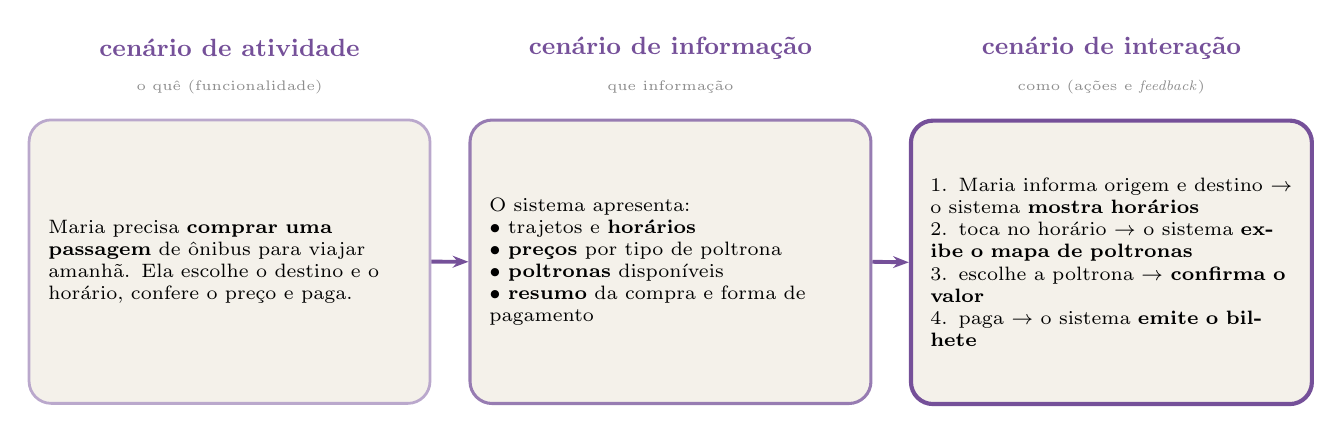
\begin{tikzpicture}[x=1cm,y=1cm,
   col/.style={dbox, rounded corners=8pt, text width=4.6cm, minimum height=3.6cm, anchor=north, align=left, font=\scriptsize, inner sep=7pt}]

  \node[font=\small\bfseries, dblue] at (2.4,0.7) {cenário de atividade};
  \node[font=\small\bfseries, dblue] at (8.0,0.7) {cenário de informação};
  \node[font=\small\bfseries, dblue] at (13.6,0.7) {cenário de interação};
  \node[dsub, font=\tiny] at (2.4,0.2) {o quê (funcionalidade)};
  \node[dsub, font=\tiny] at (8.0,0.2) {que informação};
  \node[dsub, font=\tiny] at (13.6,0.2) {como (ações e \textit{feedback})};

  \node[col, draw=dblue!50] (a) at (2.4,-0.2) {Maria precisa \textbf{comprar uma passagem} de ônibus para viajar amanhã. Ela escolhe o destino e o horário, confere o preço e paga.};
  \node[col, draw=dblue!75, line width=1.1pt] (b) at (8.0,-0.2) {O sistema apresenta:\\ $\bullet$ trajetos e \textbf{horários}\\ $\bullet$ \textbf{preços} por tipo de poltrona\\ $\bullet$ \textbf{poltronas} disponíveis\\ $\bullet$ \textbf{resumo} da compra e forma de pagamento};
  \node[col, draw=dblue, line width=1.5pt] (c) at (13.6,-0.2) {1. Maria informa origem e destino $\to$ o sistema \textbf{mostra horários}\\ 2. toca no horário $\to$ o sistema \textbf{exibe o mapa de poltronas}\\ 3. escolhe a poltrona $\to$ \textbf{confirma o valor}\\ 4. paga $\to$ o sistema \textbf{emite o bilhete}};
  \draw[dtrans, line width=1.4pt] (a.east) -- (b.west); \draw[dtrans, line width=1.4pt] (b.east) -- (c.west);


\end{tikzpicture}
\end{document}
